\documentclass{beamer}
\usepackage{hyperref}
\usepackage[T1]{fontenc}
\usepackage{algorithm2e}
\usepackage{algpseudocode}
\usepackage{bookmark}
% other packages
\usepackage{latexsym,amsmath,xcolor,multicol,booktabs,calligra}
\usepackage{graphicx,pstricks,listings,stackengine}

% dummy text; remove it when working on this template
\usepackage{lipsum}


\author{Ayush Raina}
\title{Audio Classification System using YAMNet and Wav2Vec2 Models}
\subtitle{Front-Era Health Assessment Challenge}
\institute{
    Indian Institute of Science \\
}
\date{\today}
\usepackage{Ritsumeikan}


% defs
\def\cmd#1{\texttt{\color{red}\footnotesize $\backslash$#1}}
\def\env#1{\texttt{\color{blue}\footnotesize #1}}
\definecolor{deepblue}{rgb}{0,0,0.5}
\definecolor{deepred}{RGB}{153,0,0}
\definecolor{deepgreen}{rgb}{0,0.5,0}
\definecolor{halfgray}{gray}{0.55}

\lstset{
    basicstyle=\ttfamily\small,
    keywordstyle=\bfseries\color{deepblue},
    emphstyle=\ttfamily\color{deepred},    % Custom highlighting style
    stringstyle=\color{deepgreen},
    numbers=left,
    numberstyle=\small\color{halfgray},
    rulesepcolor=\color{red!20!green!20!blue!20},
    frame=shadowbox,
}

\begin{document}

\begin{frame}
    \titlepage
\end{frame}

\section*{Dataset}
\begin{frame}{Dataset}
    Due to time constraints and limited GPU Compute available we used the total of 3950 datapoints with following distribution:

    \begin{table}[h]
        \centering
        \begin{tabular}{|c|c|}
            \hline
            \textbf{Class} & \textbf{Number of Datapoints} \\
            \hline
            Cry & 457 \\
            \hline
            Not Screaming & 2631 \\
            \hline
            Screaming & 862 \\
            \hline
        \end{tabular}
    \end{table}

    I was not able to download the other datasets whose links were provided in the challenge description, so I proceeded with the above dataset.
\end{frame}

\begin{frame}{Splitting the Dataset}
    We did the following splits:
    \begin{itemize}
        \item Train: 70\%
        \item Validation: 15\%
        \item Test: 15\%
    \end{itemize}   

    Following are the number of datapoints in each split per class:
    \begin{table}[h]
        \centering
        \begin{tabular}{|c|c|c|c|}
            \hline
            \textbf{Class} & \textbf{Train} & \textbf{Validation} & \textbf{Test} \\
            \hline
            Cry & 320 & 69 & 68 \\
            \hline
            Not Screaming & 1842 & 394 & 395 \\
            \hline
            Screaming & 603 & 129 & 130 \\
            \hline
        \end{tabular}
    \end{table}
    
\end{frame}


\section*{YAMNet Model}
\begin{frame}{YAMNet Model}

    \textbf{YAMNet Model} \\
    1. Waveform creation using librosa library, sample rate = 16kHz \\
    2. Extracting embeddings which will be used to finetune the model. \\
    
    \bigskip 

    \textbf{Technique Used} \\
    I performed transfer learning instead of finetuning the model from scratch. Transfer Learning gave better results. Embeddings are output of the model before the final layer. I used these embeddings to train a simple feedforward neural network to get our final model. 
\end{frame}

\begin{frame}{Results}
    Here are the results of the YAMNet Model:
    \begin{table}[h]
        \centering
        \begin{tabular}{|c|c|c|c|}
            \hline
            \textbf{Model} & \textbf{Train Accuracy} & \textbf{Validation Accuracy} & \textbf{Test Accuracy} \\
            \hline
            YAMNet & 97.2\% & 91.5\% & 91.2\% \\
            \hline
        \end{tabular}
    \end{table}

    \textbf{Loss Function Used:} Sparse Category CrossEntropyLoss \\
    \textbf{Optimizer Used:} Adam \\
    \textbf{Learning Rate:} 0.0005 (default with Adam) \\
    \textbf{Batch Size:} 32 \\
\end{frame}

\begin{frame}{Results}
    
    \begin{figure}
        \centering
        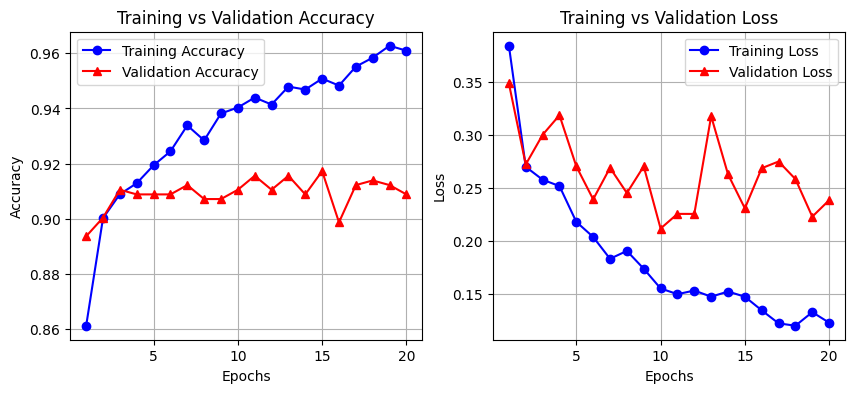
\includegraphics[width=0.8\textwidth]{yamnet1.png}
        \caption{Training Curves}
    \end{figure}

\end{frame}

\begin{frame}{Results}
    
    \begin{figure}
        \centering
        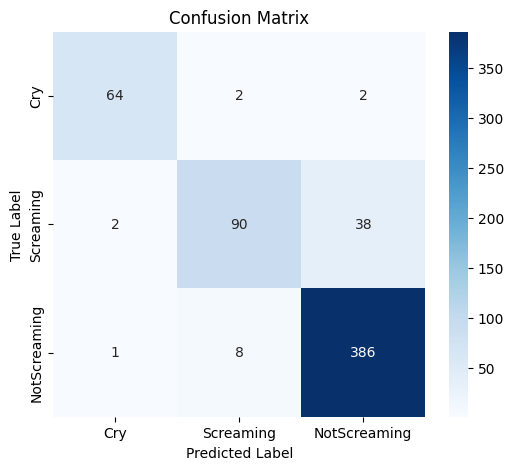
\includegraphics[width=0.6\textwidth]{yamnet2.png}
        \caption{Confusion Matrix of YAMNet Model}
    \end{figure}

\end{frame}

\begin{frame}{Results}
    
    \begin{figure}
        \centering
        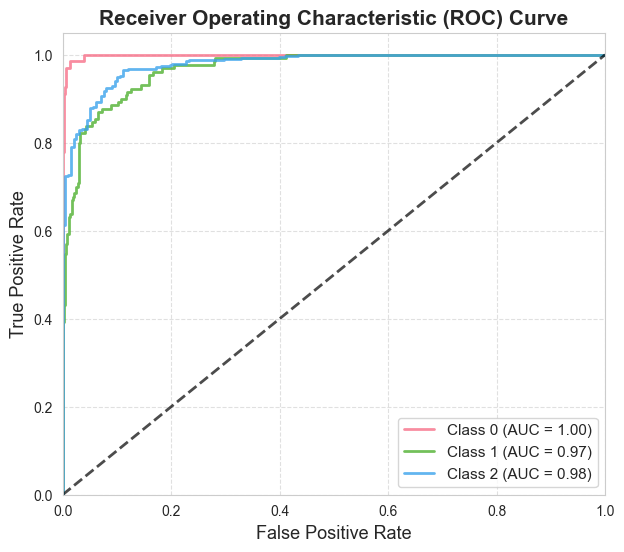
\includegraphics[width=0.6\textwidth]{yamnet3.png}
        \caption{ROC AUC Curve of YAMNet Model}
    \end{figure}

\end{frame}

\begin{frame}{Results}
    
    \begin{figure}
        \centering
        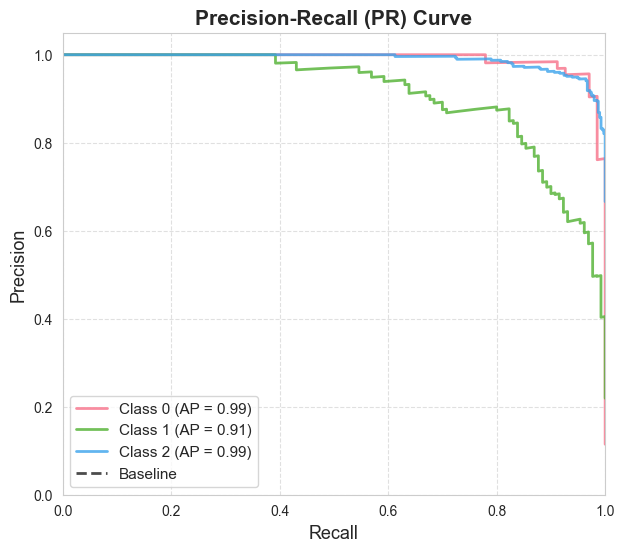
\includegraphics[width=0.6\textwidth]{yamnet4.png}
        \caption{PR Curve of YAMNet Model}
    \end{figure}

\end{frame}

\section*{Wav2Vec2 Model}
\begin{frame}{Wav2Vec2 Model}

    \textbf{Wav2Vec2 Model} \\
    1. Waveform creation using torchaudio library, sample rate = 16kHz \\
    2. Here again I used transfer learning by freezing the model and training the multi-layer perceptron on top of it. \\
    3. If 2 channels are present, I combined them to get a single channel by taking the mean of the two channels. \\
    
\end{frame}

\begin{frame}{Results}
    Here are the results of the Wav2Vec2 Model:
    \begin{table}[h]
        \centering
        \begin{tabular}{|c|c|c|c|}
            \hline
            \textbf{Model} & \textbf{Train Accuracy} & \textbf{Validation Accuracy} & \textbf{Test Accuracy} \\
            \hline
            Wav2Vec2 & 99.17\% & 90.2\% & 91.07\% \\
            \hline
        \end{tabular}
    \end{table}

    \textbf{Loss Function Used:} CrossEntropyLoss \\
    \textbf{Optimizer Used:} Adam \\
    \textbf{Learning Rate:} 0.0001 \\
    \textbf{Batch Size:} 32 \\

\end{frame}

\begin{frame}{Results}
    
    \begin{figure}
        \centering
        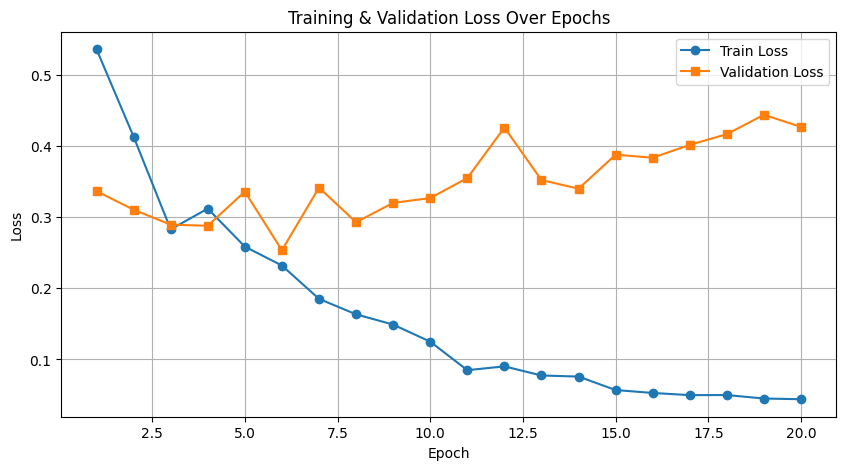
\includegraphics[width=0.8\textwidth]{wav1.png}
        \caption{Training Curve 1}
    \end{figure}

\end{frame}

\begin{frame}{Results}
    
    \begin{figure}
        \centering
        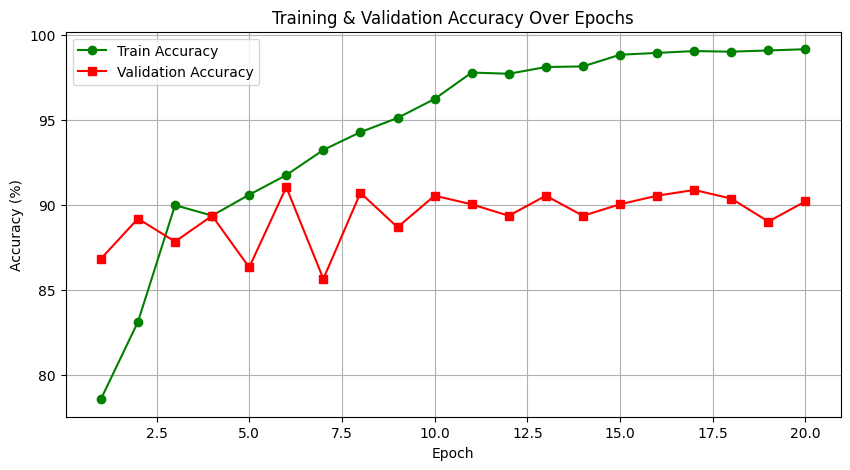
\includegraphics[width=0.8\textwidth]{wav2.png}
        \caption{Training Curve 2}
    \end{figure}

\end{frame}

\begin{frame}{Results}
    
    \begin{figure}
        \centering
        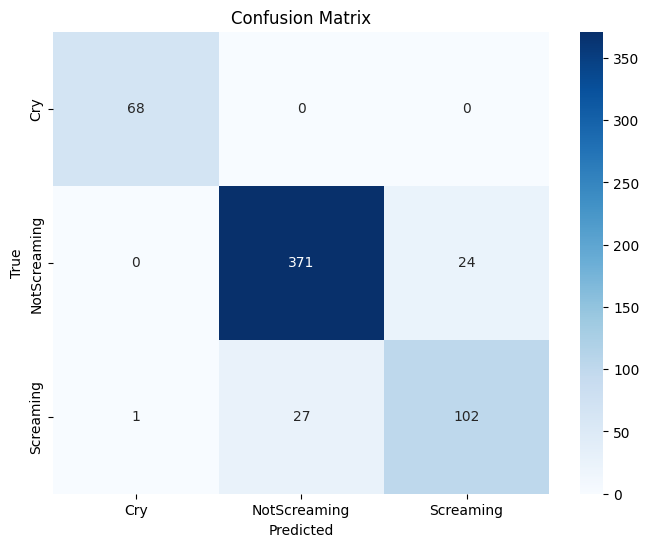
\includegraphics[width=0.6\textwidth]{wav3.png}
        \caption{Confusion Matrix of Wav2Vec2 Model}
    \end{figure}

\end{frame}

\begin{frame}{Results}
    
    \begin{figure}
        \centering
        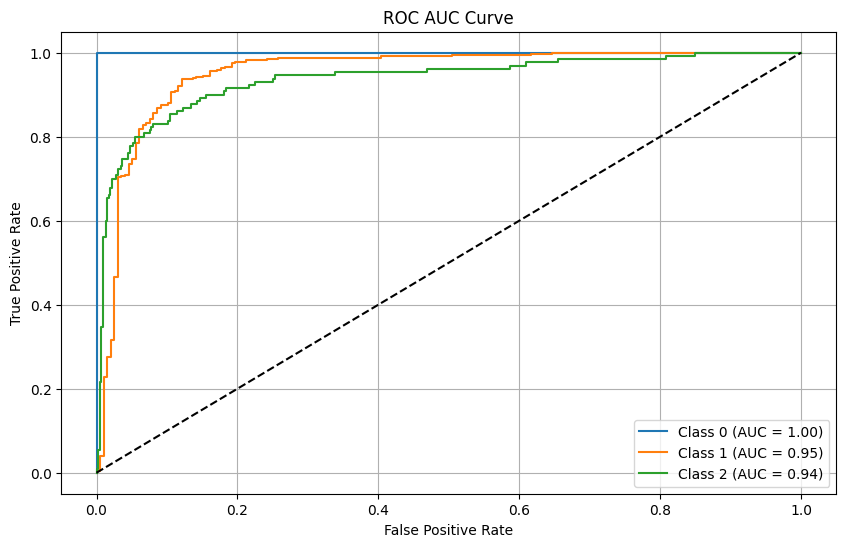
\includegraphics[width=0.6\textwidth]{wav4.png}
        \caption{ROC AUC Curve of Wav2Vec2 Model}
    \end{figure}

\end{frame}

\begin{frame}{Results}
    
    \begin{figure}
        \centering
        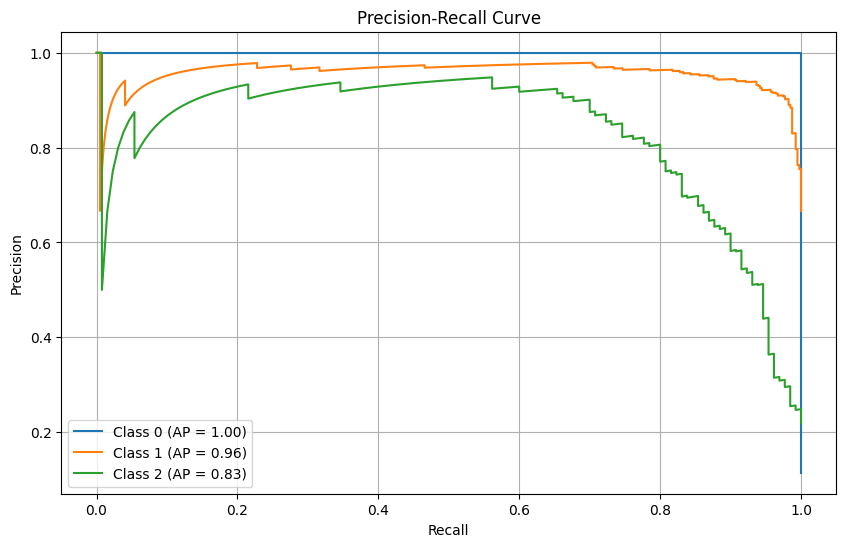
\includegraphics[width=0.6\textwidth]{wav5.png}
        \caption{PR Curve of Wav2Vec2 Model}
    \end{figure}

\end{frame}

% thank you slide
\begin{frame}{Thank You!}
    \begin{center}
        \Huge Thank You! 
    \end{center}
\end{frame}


\end{document}

